\section{Topic}
\label{sec:topic}



\subsection{Notation}
Throughout this Chapter the following notation is used:
\begin{itemize}
    \item $ \phi $ is a \emph{conjunction} of DL constraints.
    It is being checked for SAT.
    \item $ x - y \prec c $ is a general form
    of a DL constraint in $ \phi $ where $ \prec \; \in \{ <, \leq \} $.
    \item $ \mathbb{D} $ is a domain over which
    the variables and constants in $ \phi $ are defined
    (\eg $ \mathbb{R} $).
\end{itemize}



\subsection{Constraint Graph}
\begin{figure}[htb]
    \begin{center}
        \begin{tabular}{cc}
            \begin{minipage}{0.45\linewidth}
                \begin{center}
                    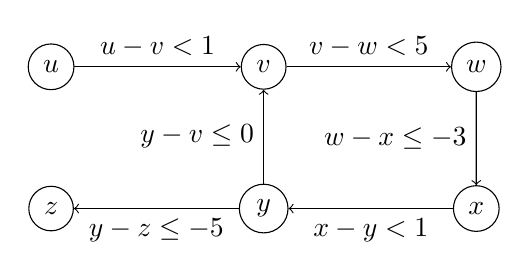
\begin{tikzpicture}[scale=0.9,state/.style={draw, circle, fill=none,text centered, text=black}]
    \node[state] (u) at (0, 2) {$u$};
    \node[state] (v) at (3, 2) {$v$};
    \node[state] (w) at (6, 2) {$w$};
    \node[state] (x) at (6, 0) {$x$};
    \node[state] (y) at (3, 0) {$y$};
    \node[state] (z) at (0, 0) {$z$};
    \draw [->] (u) -- node[anchor=south] {$ u-v < 1 $} (v);
    \draw [->] (v) -- node[anchor=south] {$ v-w < 5 $} (w);
    \draw [->] (w) -- node[anchor=east] {$ w-x \leq -3 $} (x);
    \draw [->] (x) -- node[anchor=north] {$ x-y < 1 $} (y);
    \draw [->] (y) -- node[anchor=north] {$ y-z \leq -5 $} (z);
    \draw [->] (y) -- node[anchor=east] {$ y-v \leq 0 $} (v);
\end{tikzpicture}

                \end{center}
            \end{minipage}
            &
            \begin{minipage}{0.45\linewidth}
                \begin{center}
                    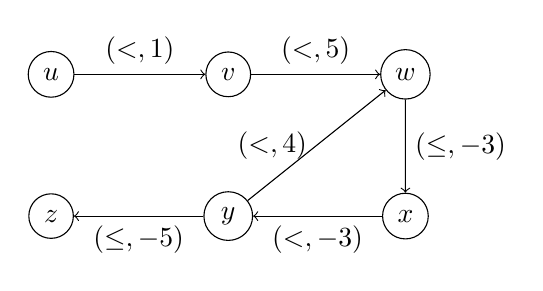
\begin{tikzpicture}[scale=0.9,state/.style={draw, circle, fill=none,text centered, text=black}]
    \node[state] (u) at (0, 2) {$u$};
    \node[state] (v) at (2.5, 2) {$v$};
    \node[state] (w) at (5, 2) {$w$};
    \node[state] (x) at (5, 0) {$x$};
    \node[state] (y) at (2.5, 0) {$y$};
    \node[state] (z) at (0, 0) {$z$};
    \draw [->] (u) -- node[anchor=south] {$ (<,1) $} (v);
    \draw [->] (v) -- node[anchor=south] {$ (<,5) $} (w);
    \draw [->] (w) -- node[anchor=west] {$ (\leq,-3) $} (x);
    \draw [->] (x) -- node[anchor=north] {$ (<,-3) $} (y);
    \draw [->] (y) -- node[anchor=north] {$ (\leq,-5) $} (z);
    \draw [->] (y) -- node[anchor=east] {$ (<,4) $} (w);
\end{tikzpicture}

                \end{center}
            \end{minipage}
        \end{tabular}
    \end{center}
    \caption{Examples of constraint graphs for
        Equation~\ref{eq:example-2} (left) and
        Equation~\ref{eq:example-3} (right).}
    \label{fig:contraints-graphs}
\end{figure}
Constraint graph (Figure~\ref{fig:contraints-graphs})
is a weighted directed graph which represents $ \phi $
and which is used by a DL constraints checker
(Figure~\ref{fig:lazy-and-incremental-approaches}) to test
if $ \phi $ is SAT.
In~\cite{cotton2004some} it is defined as follows:
\begin{definition}[Constraint Graph]
    \label{def:constraint-graph}
    The constraint graph is a graph $ \Gamma = (V,E,weight,op) $ where:
    \begin{itemize}
        \item $ V $ is a set of vertices. Each vertex $ x \in V $
        corresponds to one numeric variable occurring in $ x - y \prec c $.
        \item $ E $ is a set of directed edges. Each edge
        $ (x,y) \in E $ corresponds to $ x - y \prec c $.
        \item $ weight(x,y): E \mapsto \mathbb{D} $ is a weight function.
        It maps each edge $ (x,y) \in E $ to the constant
        $ c \in \mathbb{D} $ from the corresponding DL inequality
        $ x - y \prec c $.
        \item $ op(x,y): E \mapsto \{ <, \leq \} $ is a function which
        maps each edge $ (x,y) \in E $ to the operation
        $ \prec $ from the corresponding DL inequality
        $ x - y \prec c $.
    \end{itemize}
\end{definition}




\subsection{Negative Cycles in Constraint Graph}
There is a direct correspondence between a negative cycle
in a constraint graph and SAT of $ \phi $ represented by this graph.

A path in the graph corresponds to a sum of the corresponding
constraints. \Eg the path
$ u \rightarrow v \rightarrow w \rightarrow x $
in the left graph on Figure~\ref{fig:contraints-graphs}
corresponds to the following sum of the DL inequalities:
\begin{equation}
    \begin{aligned}
        u - v & < \;\;\; 1 \\
        v - w & < \;\;\; 5 \\
        w - x & \leq -3 \\
        \hline
        u - x & < \;\;\; 3
    \end{aligned}
\end{equation}
If at least one strict inequality is present
then the resulting inequality will also be strict.
This summation along a path can also be expressed with
an inferred transitivity constraint
(\eg~Equation~\ref{eq:transitivity-example}).
The transitivity constraint naturally follows from $ \phi $ and
therefore must be satisfied in order to satisfy $ \phi $.

A cycle in the constraint graph corresponds to an inequality
$ 0 \prec c $
which may cause a conflict in the following situations:
\begin{itemize}
    \item $ c < 0$
    \item $ c = 0 $ and $ \prec $ is $ < $
    (can be checked with $ op $ from Definition~\ref{def:constraint-graph})
\end{itemize}

An example of a conflict can be seen on the right graph
on Figure~\ref{fig:contraints-graphs}.
The conflict corresponds to the negative cycle
$ x \rightarrow y \rightarrow w \rightarrow x $
which corresponds to the following conflicting inequalities:
\begin{equation}
    \begin{aligned}
        x - y & < -3 \\
        y - w & < \;\;\; 4 \\
        w - x & \leq -3 \\
        \hline
        0 & < -2
    \end{aligned}
\end{equation}



\subsection{Bellman-Ford Algorithm for Constraint Graph}
\cite{cotton2004some} uses a Goldberg-Radzik~\cite{goldberg1993heuristic}
variant of the Bellman-Ford algorithm~\cite[p.651]{cormen2009introduction}
to detect negative cycles
and thus check $ \phi $ for SAT
(Algorithm~\ref{alg:goldberg-radzik}).
\cite{goldberg1993heuristic}~states that the algorithm has the same
worst-case complexity $ O(|V| \cdot |E|) $
as Bellman-Ford algorithm but is superior in practice.
Terminology and notation used in the algorithm are given below.

\begin{Algorithm}
    \caption{An algorithm for checking if $ \phi $ which corresponds
        to the input constraint graph $ \Gamma = (V,E,weight,op) $ is SAT.
        It returns SAT or UNSAT status and a set of DL constraints
        corresponding to a conflict (in case of UNSAT).
        It is based on Bellman-Ford
        algorithm~\cite[p.561]{cormen2009introduction}.
        Goldberg-Radzik heuristic~\cite{goldberg1993heuristic},
        which is used here,
        suggests to scan a graph in a topological order.
        This algorithm uses
        depth first search~\cite[p.603]{cormen2009introduction} (DFS)
        and breadth first search~\cite[p.594]{cormen2009introduction} (BFS)
        for auxiliary tasks.}
    \label{alg:goldberg-radzik}
    \begin{algorithm}{Goldberg-Radzik}
        {\text{constraint graph} \Gamma = (V,E,weight,op),
            \text{source vertex} s \in V}
        \begin{FOR}{\mathrm{each \; vertex} \; x \in V}
            d(x) = \infty \\
            status(x) = unreached
        \end{FOR} \\
        d(s) = 0 \\
        status(s) = labeled \\
        A \= \varnothing \\
        B \= \{ s \} \\
        \begin{REPEAT} \\
            \begin{IF}{\Gamma_d \text{has a cycle} C \text{(DFS on} \Gamma_d \text{can be used to check it)}}
                l \= \text{length of} C \text{in} \Gamma \\
                \begin{IF}{l < 0}
                    \RETURN (UNSAT, \text{DL constraints corresponding to} L)
                \end{IF} \\
                \begin{IF}{\exists \; (x,y) \in L \text{such that} op(x,y) = \; <}
                    \RETURN (UNSAT, \text{DL constraints corresponding to} L)
                \end{IF}
            \end{IF} \\
            \begin{FOR}{\mathrm{each \; vertex} \; x \in B}
                \begin{IF}{x \text{has no outgoing admissible edges}}
                    B \= B \setminus \{ x \} \\
                    status(x) = scanned
                \end{IF}
            \end{FOR} \\
            A \= \text{set of unexplored vertices reachable from}
            B \text{in} \Gamma_d
            \text{(BFS on} \Gamma_d \text{can be used here)} \\
            A \= \text{sort} A \text{topologically using}
            \Gamma_d \text{as an input graph}
            \text{(DFS on} \Gamma_d \text{can be used here)} \\
            B \= \varnothing \\
            \begin{FOR}{\mathrm{each \; vertex} \; x \in A}
                status(x) = labeled \\
                \begin{FOR}{\mathrm{each \; edge} \; (x,y) \in E}
                    \begin{IF}{d(x) + weight(x,y) < d(y)}
                        d(y) \= d(x) + weight(x,y) \\
                        \begin{IF}{status(y) = unreached}
                            B \= B \cup \{ y \}
                        \end{IF} \\
                        status(y) \= labeled \\
                        status(x) \= scanned
                    \end{IF}
                \end{FOR}
            \end{FOR}
        \end{REPEAT} A \; is \; empty \\
        \RETURN (SAT, \varnothing) \\
    \end{algorithm}
\end{Algorithm}

\begin{definition}[Source Vertex]
    The source vertex $ s \in V $ is a vertex from which
    the shortest paths to other vertices are computed.
\end{definition}

\begin{definition}[Distance Estimating Function~\cite{cotton2004some}]
    The distance estimating function $ d(v): V \mapsto \mathbb{D} $
    is a function which returns an upper bound
    on the length of the shortest path
    from the source vertex to the given vertex $ v \in V $.
\end{definition}

\begin{definition}[Reduced Cost Function~\cite{goldberg1993heuristic}]
    The reduced cost function
    $ r(x,y): V \mapsto \mathbb{D} $ is
    defined as follows:
    $ r(x,y) = weight(x,y) + d(x) - d(y) $.
\end{definition}

\newpage

\begin{definition}[Vertex Status]
    The vertex status
    $ status(x) = \{ unreached, labeled, scanned \} $
    is a function on vertices which shows a current state of
    a vertex $ x \in V $.
    $ status(x) = unreached $ means $ x $ has not been explored yet.
    $ status(x) = labeled $ means $ x $ has been explored \ie
    the distance estimate for it has been updated at least once
    and potentially it can be used to improve distance estimates to
    other vertices.
    $ status(x) = scanned $ means $ x $ has been completely explored
    and will not be considered further for improving distance estimates.
\end{definition}
\begin{definition}[Admissible Edge]
    Edge $ (x,y) \in E $ is called admissible if $ r_d(x,y) \leq 0 $.
\end{definition}
\begin{definition}[Admissible Graph]
    Admissible graph $ \Gamma_d $ is a subgraph
    of $ \Gamma $ composed of the admissible edges of $ \Gamma $.
\end{definition}

In Algorithm~\ref{alg:goldberg-radzik} distance estimates are iteratively
updated.
In~\cite[p.648]{cormen2009introduction} the act of updating a distance
estimate using an edge is called ``edge relaxation``
(Equation~\ref{eq:edge-relaxation}).
This iterative process can also be seen as a series of different distance
estimating functions $ (d_0, d_1, d_2, d_3, \dots) $.
Each $ d_i $ in this series describes which distance estimates
have the vertices at some iteration of
the Algorithm~\ref{alg:goldberg-radzik}.

\begin{figure}[htb]
    \begin{center}
        \begin{tabular}{c}
            \begin{minipage}{0.95\linewidth}
                \begin{center}
                    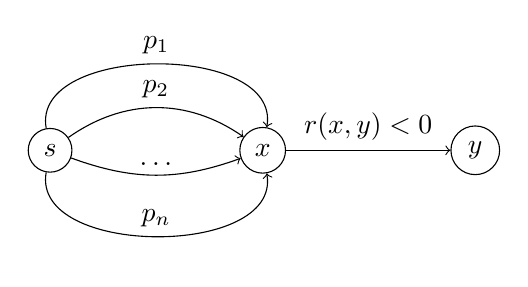
\begin{tikzpicture}[scale=0.9,state/.style={draw, circle, fill=none,text centered, text=black}]
    \node[state] (s) at (0, 0) {$s$};
    \node[state] (x) at (3, 0) {$x$};
    \node[state] (y) at (6, 0) {$y$};

    \draw [->] (x) -- node[anchor=south] {$ r(x,y) < 0 $} (y);

    \draw [->] (s) edge[bend right=-100] node[anchor=south] {$ p_1 $} (x);
    \draw [->] (s) edge[bend right=-35] node[anchor=south] {$ p_2 $} (x);
    \draw [->] (s) edge[bend right=20] node[anchor=south] {$ \dots $} (x);
    \draw [->] (s) edge[bend right=100] node[anchor=south] {$ p_n $} (x);
\end{tikzpicture}

                \end{center}
            \end{minipage}
        \end{tabular}
    \end{center}
    \caption{Multiple paths from $ s $ to $ y $
        may be used to improve distance estimate to $ x $.}
    \label{fig:edge-relaxation}
\end{figure}
The idea of the Algorithm~\ref{alg:goldberg-radzik} is to use
the dynamically changing graph $ \Gamma_d $
(it changes whenever $ d $ changes)
to detect negative or zero cycles in the original graph $ \Gamma $.
The following theorem from~\cite{cotton2004some}
expresses this idea more formally.

\begin{theorem}
    \label{the:neg-cycle-in-cg}
    Given a constraint graph $ \Gamma $ and a series of distance estimating
    functions $ (d_0, d_1, d_2, d_3, \dots) $, $ \Gamma $ has a negative
    or zero cycle if and only if $ \Gamma_d $ has a cycle under some
    distance estimate $ d_k $.
    \begin{proof}
        $ \Rightarrow $ Case 1. $ \Gamma $ has a negative cycle.
        To prove: $ \Gamma_d $ has a cycle at some distance estimate $ d_k $.

        Suppose $ \Gamma_d $ has no cycles at any distance estimate
        (the initial assumption).
        Consider an arbitrary edge $ (x,y) \in \Gamma_d $
        at some distance estimate $ d_k $ for which $ r(x,y) < 0 $
        \ie this edge can be relaxed.
        If we apply relaxation to this edge then we change the
        distance estimate to some $ d_{k+1} $ by updating
        distance estimate for the vertex $ y $ to a smaller value:
        \begin{equation}
            \label{eq:edge-relaxation}
            \begin{aligned}
                r(x,y) < 0 \Rightarrow d_k(x) + weight(x,y) < d_k(y) \\
                d_{k+1}(y) = d_k(x) + weight(x,y)
            \end{aligned}
        \end{equation}
        Immediately after this operation
        we will have that $ r(x,y) = 0 $ and thus
        the edge will still be in $ \Gamma_d $ but relaxation
        cannot be applicable to it.
        It can be the case, however, that this edge will be relaxed
        again in some further iterations.
        Since there are no cycles in $ \Gamma_d $,
        multiple updates are only possible
        when there are some better paths $ p_1, p_2, \dots p_n $
        from the source vertex $ s $
        to $ x $ (Figure~\ref{fig:edge-relaxation}).
        These paths can be used to update distance estimate
        for the vertex $ x $ and make possible relaxation
        of the edge $ (x,y) $.
        Number of these paths cannot be infinite
        because the graph has finite number of vertices and edges.
        Therefore the edge $ (x,y) $ will be relaxed finitely many
        times.
        Then $ r(x,y) $ will become zero at some iteration and
        the edge will stay in $ \Gamma_d $ for all further iterations.

        The above reasoning has been applied to an arbitrary edge
        $ (x,y) $ for which we have $ r(x,y) < 0 $ at some distance
        estimate $ d_k $ during the execution of the algorithm.
        This reasoning can be repeated for all other edges and
        it can be concluded therefore that
        after some finite number of iterations no
        distance updates will be possible, because for any edge
        $ (x,y) \in \Gamma $ we will have $ r(x,y) \ge 0 $.
        Thus, the distance update process will converge.
        However, in~\cite[p.653]{cormen2009introduction} it has been
        proven that, in case when $ \Gamma $ has a negative cycle,
        the distance update process does not converge.
        Therefore we have a contradiction and the initial assumption
        is wrong.
        Thus, $ \Gamma_d $ will have a cycle at some distance estimate.
        \\

        Case 2. $ \Gamma $ has no negative cycles but it has
        a zero weight cycle $ Z = (x_0, x_1, \dots, x_{n-1}, x_n) $
        with $ x_n = x_0 $.
        To prove: $ \Gamma_d $ has a cycle at some distance estimate $ d_k $.

        In this case the distance estimate process
        will converge to some function
        $ d_k $ which means that there is no edge that can be relaxed,
        including the edges of $ Z $:
        \begin{equation}
            \label{eq:triangle-inequlity}
            d(x_i) + weight(x_i, x_{i+1}) \ge d(x_{i+1}), \; 0 \le i < n
        \end{equation}
        Let us sum the inequality from Equation~\ref{eq:triangle-inequlity}
        along the cycle $ Z $:
        \begin{equation}
            \label{eq:sum-along-cycle}
            \begin{aligned}
                \sum_{i=0}^{n-1} d(x_i) + \sum_{i=0}^{n-1} weight(x_i, x_{i+1}) \ge \sum_{i=0}^{n-1} d(x_{i+1}) \\
                \sum_{i=0}^{n-1} weight(x_i, x_{i+1}) \ge \sum_{i=0}^{n-1} d(x_{i+1}) - \sum_{i=0}^{n-1} d(x_i) \\
                Z \; \mathrm{has \; zero \; weight} \\
                0 \ge \sum_{i=0}^{n-1} d(x_{i+1}) - \sum_{i=0}^{n-1} d(x_i) \\
                \mathrm{apply \; index \; renaming \; to \; the \; first \; sum} \\
                0 \ge \sum_{i=1}^{n} d(x_i) - \sum_{i=0}^{n-1} d(x_i) \\
                \mathrm{since} \; x_0 = x_n \; \mathrm{the \; two \; sums \; are \; actually \; equal} \\
                0 \ge 0
            \end{aligned}
        \end{equation}
        The final inequality in Equation~\ref{eq:sum-along-cycle}
        is valid and is a consequence of the convergence.

        Now assume that there is at least one edge
        $ (x_i,x_{i+1}) $
        along the cycle $ Z $
        for which we have
        $ d(x_i) + weight(x_i, x_{i+1}) > d(x_{i+1}) $
        (the initial assumption).
        Then, if we do the summation
        in Equation~\ref{eq:sum-along-cycle} again,
        we will get a strict inequality $ 0 > 0 $
        which is invalid.
        Thus, we have a contradiction with the convergence condition
        and therefore the initial assumption is invalid.
        Thus
        $ d(x_i) + weight(x_i, x_{i+1}) = d(x_{i+1}), \; 0 \le i < n $
        and $ r(x_i, x_{i+1}) = 0 $
        and therefore all edges of $ Z $ are admissible
        and they are in the graph $ \Gamma_d $.
        \\

        $ \Leftarrow $ $ \Gamma_d $ under some distance estimate $ d_k $
        has a cycle
        $ C = (x_0, x_1, \dots, x_{n-1}, x_n) $ with $ x_0 = x_n $.
        To prove: there is a negative or zero weight cycle in $ \Gamma $.

        $ C $ is in the graph $ \Gamma_d $.
        Therefore its edges are admissible:
        \begin{equation}
            \label{eq:cycle-sum}
            \begin{aligned}
                r(x_i, x_{i+1}) \le 0, \; 0 \le i < n \\
                d(x_i) + weight(x_i, x_{i+1}) - d(x_{i+1}) \le 0, \; 0 \le i < n \\
                d(x_i) + weight(x_i, x_{i+1}) \le d(x_{i+1}), \; 0 \le i < n \\
                \mathrm{apply \; summation \; along \; the \; cycle} \\
                \sum_{i=0}^{n-1} d(x_i) + \sum_{i=0}^{n-1} weight(x_i, x_{i+1}) \le \sum_{i=0}^{n-1} d(x_{i+1}) \\
                 \sum_{i=0}^{n-1} weight(x_i, x_{i+1}) \le \sum_{i=0}^{n-1} d(x_{i+1}) - \sum_{i=0}^{n-1} d(x_i) \\
                 \mathrm{the \; two \; sums \; on \; the \; right \; are \; equal \; (see \; Equation~\ref{eq:sum-along-cycle})} \\
                 \sum_{i=0}^{n-1} weight(x_i, x_{i+1}) \le 0 \\
            \end{aligned}
        \end{equation}
        The left hand side expression in the final inequality
        in Equation~\ref{eq:cycle-sum} is the length of the cycle $ C $
        which is less than or equal to zero.
    \end{proof}
\end{theorem}
